\begin{flushleft}
	\section{\textcolor{cyan}{Généralité sur la maison intelligente}}
	\subsection{\textcolor{green}{Historique de la domotique :}}
	Brièvement, le mot domotique a été introduit dans le dictionnaire « le
	petit Larousse » en 1988. Ce mot a été construit à partir de « Domus »,
	la demeure de maître en latin, associé au suffixe « tique », couramment
	employé pour évoquer le terme des technologies (automatique,
	électronique, électrique, informatique). On associe souvent le début des
	travaux domotiques aux années 1970, voire 1980, avec les
	problématiques énergétiques dues aux crises pétrolières qui ont
	considérablement affecté le domaine de la construction et de
	l’exploitation du bâtiment. Depuis le milieu des années 1990, un autre
	segment, orienté sur la microinformatique et les loisirs numériques, se
	développe. Cette nouvelle apparition marque en particulier
	l’introduction de l’informatique dans l’habitat et l’apparition des
	supports numériques : les cédéroms, puis les DVD et internet. Ainsi
	aujourd’hui, la gestion de l’habitat, la sécurité, les réseaux de
	communication et les loisirs numériques esquissent le paradigme de
	domotique.
	\subsection{\textcolor{green}{La maison intelligente :}}
	 La maison intelligente est une maison avec des fonctions qui
	 simplifient le quotidien de ses habitants, pour générer de l'énergie et
	 assurer certaines fonctions avec un certain degré de confort de toiture et de sécurité. Elle est en constante évolution et s'ouvrant sur le monde.
	 C’est un mot récent de la langue française et il est en réalité la somme
	 des mots « doums » qui signifient domicile en latin et du suffixe « tique » rattaché au mot technique.
	 \begin{figure}[h]
	 	\centering
	 	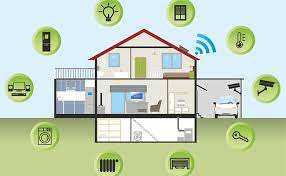
\includegraphics{chapitres/images/SmartHome.jpg}
	 	\caption{La maison intelligente}
	 	\label{fig:labelname}
	 \end{figure}
  La maison intelligente utilise plusieurs critères clés : la sécurité, le confort de vie, les économies d’énergies et la santé et la communication.
 	\subsection{\textcolor{green}{La sécurité:}}
 	Le système domotique offre une protection complète des biens et des personnes grâce à l'utilisation de capteurs pour détecter les intrusions, surveiller les accès et détecter les anomalies techniques telles que les fuites d'eau ou les incendies. Les occupants peuvent recevoir des alertes en temps réel par e-mail ou sur leur téléphone portable en cas d'incident potentiel, ce qui leur permet de prendre des mesures pour protéger leur propriété et leur sécurité.
 	\subsection{\textcolor{green}{Le confort :}}
 	En utilisant un smartphone,la maison intelligente est
 	capable de savoir quand vous rentrez à la maison et donc d’ouvrir le
 	portail avant même que vous n’arriviez. Les volets peuvent s’ouvrir et
 	se fermer au rythme du soleil, et peuvent même aller jusqu’à
 	s’adapter à la saison et la température pour laisser entrer la lumière et
 	la chaleur du soleil l’hiver, ou au contraire conserver le frais l’été en
 	fermant les volets des fenêtres exposées au soleil.
 	\subsection{\textcolor{green}{La santé :}}
 	La maison intelligente trouve aujourd’hui de nouvelles applications dans le
 	domaine de la santé. Afin d’améliorer l’autonomie et l’indépendance
 	des personnes fragiles, handicapées ou âgées le souci de leurs mises
 	en garde à distance chez eux peut être maintenant possible.
 	\subsection{\textcolor{green}{L’économie d’énergie :}}
 	En gérant les volets selon la saison, ainsi que le chauffage, le système
 	domotique vous permet d’économiser de l’énergie, et donc de
 	l’argent, même si au départ on ne recherchait que le confort en plus.
 	La consommation d’énergie peut être suivie très finement, qu’il
 	s’agisse de votre consommation d’électricité, d’eau, ou même de gaz.
 	\subsection{\textcolor{green}{La communication :}}
 	La communication dans la maison intelligente est Le
 	mariage de l'informatique, des télécom et l'électronique. Au royaume
 	des normes domotique, il est difficile de se retrouver. On trouve des
 	types différents de la communication dans la smart house comme montre le figure ci dessous .
 	\begin{figure}[h]
 		\centering
 		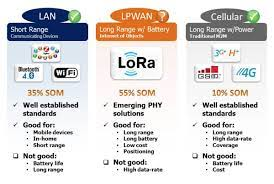
\includegraphics{chapitres/images/communication.jpg}
 		\caption{Les différents protocoles de communication sans fil}
 		\label{fig:labelname}
 	\end{figure}
 	\subsection{\textcolor{green}{Conclusion :}}
 	La maison intelligente est une maison équipée de fonctions automatisées qui simplifient le quotidien de ses habitants en termes de sécurité, de confort, d'économies d'énergie, de santé et de communication. Elle utilise des capteurs pour détecter les intrusions, surveiller les accès et prévenir les incidents tels que les fuites d'eau ou les incendies. En termes de confort, la maison intelligente peut s'adapter à la saison et à la température pour laisser entrer la lumière et la chaleur du soleil en hiver ou conserver la fraîcheur en été. Elle peut également être utilisée pour améliorer l'autonomie des personnes fragiles, handicapées ou âgées. En gérant les volets et le chauffage, la maison intelligente permet également des économies d'énergie. Enfin, la communication est également intégrée à la maison intelligente grâce à l'informatique, les télécommunications et l'électronique.
 	
 	\newpage
\end{flushleft}
